%===============================================================================
% LaTeX sjabloon voor de bachelorproef toegepaste informatica aan HOGENT
% Meer info op https://github.com/HoGentTIN/bachproef-latex-sjabloon
%===============================================================================

\documentclass{bachproef-tin}

\usepackage{hogent-thesis-titlepage} % Titelpagina conform aan HOGENT huisstijl

%%---------- Documenteigenschappen ---------------------------------------------
% TODO: Vul dit aan met je eigen info:

% De titel van het rapport/bachelorproef
\title{Titel}

% Je eigen naam
\author{Arno Boel}

% De naam van je promotor (lector van de opleiding)
\promotor{Martine Van Audenrode}

% De naam van je co-promotor. Als je promotor ook je opdrachtgever is en je
% dus ook inhoudelijk begeleidt (en enkel dan!), mag je dit leeg laten.
\copromotor{Stijn De Smet}

% Indien je bachelorproef in opdracht van/in samenwerking met een bedrijf of
% externe organisatie geschreven is, geef je hier de naam. Zoniet laat je dit
% zoals het is.
\instelling{Zoovu}

% Academiejaar
\academiejaar{2019-2020}

% Examenperiode
%  - 1e semester = 1e examenperiode => 1
%  - 2e semester = 2e examenperiode => 2
%  - tweede zit  = 3e examenperiode => 3
\examenperiode{2}

%===============================================================================
% Inhoud document
%===============================================================================

\begin{document}

%---------- Taalselectie -------------------------------------------------------
% Als je je bachelorproef in het Engels schrijft, haal dan onderstaande regel
% uit commentaar. Let op: de tekst op de voorkaft blijft in het Nederlands, en
% dat is ook de bedoeling!

%\selectlanguage{english}

%---------- Titelblad ----------------------------------------------------------
\inserttitlepage

%---------- Samenvatting, voorwoord --------------------------------------------
\usechapterimagefalse
%%=============================================================================
%% Voorwoord
%%=============================================================================

\chapter*{\IfLanguageName{dutch}{Woord vooraf}{Preface}}
\label{ch:voorwoord}

%% TODO:
%% Het voorwoord is het enige deel van de bachelorproef waar je vanuit je
%% eigen standpunt (``ik-vorm'') mag schrijven. Je kan hier bv. motiveren
%% waarom jij het onderwerp wil bespreken.
%% Vergeet ook niet te bedanken wie je geholpen/gesteund/... heeft


%%=============================================================================
%% Samenvatting
%%=============================================================================

% TODO: De "abstract" of samenvatting is een kernachtige (~ 1 blz. voor een
% thesis) synthese van het document.
%
% Deze aspecten moeten zeker aan bod komen:
% - Context: waarom is dit werk belangrijk?
% - Nood: waarom moest dit onderzocht worden?
% - Taak: wat heb je precies gedaan?
% - Object: wat staat in dit document geschreven?
% - Resultaat: wat was het resultaat?
% - Conclusie: wat is/zijn de belangrijkste conclusie(s)?
% - Perspectief: blijven er nog vragen open die in de toekomst nog kunnen
%    onderzocht worden? Wat is een mogelijk vervolg voor jouw onderzoek?
%
% LET OP! Een samenvatting is GEEN voorwoord!

%%---------- Nederlandse samenvatting -----------------------------------------
%
% TODO: Als je je bachelorproef in het Engels schrijft, moet je eerst een
% Nederlandse samenvatting invoegen. Haal daarvoor onderstaande code uit
% commentaar.
% Wie zijn bachelorproef in het Nederlands schrijft, kan dit negeren, de inhoud
% wordt niet in het document ingevoegd.

\IfLanguageName{english}{%
\selectlanguage{dutch}
\chapter*{Samenvatting}
\selectlanguage{english}
}{}

%%---------- Samenvatting -----------------------------------------------------
% De samenvatting in de hoofdtaal van het document

\chapter*{\IfLanguageName{dutch}{Samenvatting}{Abstract}}

De hedendaagse wereld draait steeds meer en meer rond technologie. Mensen shoppen steeds vaker bij webshops, zoeken op websites naar bepaade informatie of willen een klantendienst online bereiken. Een service die vele bedrijven daarom aanbieden is de mogelijkheid om op hun website/webshop te kunnen chatten met een medewerker die hun specifieke vragen kan beantwoorden. Om de grote toevloed aan chatberichten de baas te kunnen kiezen vele bedrijven voor een chatbot als eerste aanpsreekpunt voor een klant. Deze kan reeds veel informatie bekomen door met de klant in gesprek te gaan. Een chatbot werkt volledig automatisch en ontlast zodoende de medewerkers van het bedrijf. 

Aangezien een chatbot volledig autonoom moet kunnen werken is het noodzakelijk om de kwaliteit van de chatbot te kunnen garanderen. Om zich er van te vergewissen dat de chatbot aan de eisen voldoet en zinvolle antwoorden geeft op de input van gebruikers maken ontwikkelaars gebruik van testen. Deze testen worden geschreven op hetzelfde moment als dat de code voor die bepaalde feature geschreven wordt. Op dat moment kan er dus met zekerheid gezegd worden dat die bepaalde feature voldoet aan de kwaliteitseisen die gesteld worden en kan de chatbot opgeleverd worden met deze nieuwe feature. 

Zoals in elk software project komen er ook bij een chatbot voortdurend nieuwe features bij. Dit kan bijvoorbeeld gaan over het toevoegen van een nieuwe taal die ondersteund wordt, bepaalde onderwerpen toevoegen die de chatbot verder kan beantwoorden, extra taken opnemen dan louter informatie geven, ... Er zijn enorm veel mogelijkheden om uit te breiden. Al deze uitbreidingen moeten ook op hun beurt getest worden en mogen andere reeds werkende features natuurlijk niet kapot gaan maken. Dit is waar regressie testen aan bod komt: het uitvoeren van testen van eerder geschreven features zodat deze nog steeds werken na het toevoegen van een nieuwe feature. Op deze manier kan een ontwikkelaar er zeker van zijn dat een gebruiker dezelfde service als ervoor zal kunnen ervaren.

% Taak

%

%---------- Inhoudstafel -------------------------------------------------------
\pagestyle{empty} % Geen hoofding
\tableofcontents  % Voeg de inhoudstafel toe
\cleardoublepage  % Zorg dat volgende hoofstuk op een oneven pagina begint
\pagestyle{fancy} % Zet hoofding opnieuw aan

%---------- Lijst figuren, afkortingen, ... ------------------------------------

% Indien gewenst kan je hier een lijst van figuren/tabellen opgeven. Geef in
% dat geval je figuren/tabellen altijd een korte beschrijving:
%
%  \caption[korte beschrijving]{uitgebreide beschrijving}
%
% De korte beschrijving wordt gebruikt voor deze lijst, de uitgebreide staat bij
% de figuur of tabel zelf.

\listoffigures
\listoftables

% Als je een lijst van afkortingen of termen wil toevoegen, dan hoort die
% hier thuis. Gebruik bijvoorbeeld de ``glossaries'' package.
% https://www.overleaf.com/learn/latex/Glossaries

%---------- Kern ---------------------------------------------------------------

% De eerste hoofdstukken van een bachelorproef zijn meestal een inleiding op
% het onderwerp, literatuurstudie en verantwoording methodologie.
% Aarzel niet om een meer beschrijvende titel aan deze hoofstukken te geven of
% om bijvoorbeeld de inleiding en/of stand van zaken over meerdere hoofdstukken
% te verspreiden!

%%=============================================================================
%% Inleiding
%%=============================================================================

\chapter{\IfLanguageName{dutch}{Inleiding}{Introduction}}
\label{ch:inleiding}

De inleiding moet de lezer net genoeg informatie verschaffen om het onderwerp te begrijpen en in te zien waarom de onderzoeksvraag de moeite waard is om te onderzoeken. In de inleiding ga je literatuurverwijzingen beperken, zodat de tekst vlot leesbaar blijft. Je kan de inleiding verder onderverdelen in secties als dit de tekst verduidelijkt. Zaken die aan bod kunnen komen in de inleiding~\autocite{Pollefliet2011}:

\begin{itemize}
  \item context, achtergrond
  \item afbakenen van het onderwerp
  \item verantwoording van het onderwerp, methodologie
  \item probleemstelling
  \item onderzoeksdoelstelling
  \item onderzoeksvraag
  \item \ldots
\end{itemize}

\section{\IfLanguageName{dutch}{Probleemstelling}{Problem Statement}}
\label{sec:probleemstelling}

Uit je probleemstelling moet duidelijk zijn dat je onderzoek een meerwaarde heeft voor een concrete doelgroep. De doelgroep moet goed gedefinieerd en afgelijnd zijn. Doelgroepen als ``bedrijven,'' ``KMO's,'' systeembeheerders, enz.~zijn nog te vaag. Als je een lijstje kan maken van de personen/organisaties die een meerwaarde zullen vinden in deze bachelorproef (dit is eigenlijk je steekproefkader), dan is dat een indicatie dat de doelgroep goed gedefinieerd is. Dit kan een enkel bedrijf zijn of zelfs één persoon (je co-promotor/opdrachtgever).

\section{\IfLanguageName{dutch}{Onderzoeksvraag}{Research question}}
\label{sec:onderzoeksvraag}

Wees zo concreet mogelijk bij het formuleren van je onderzoeksvraag. Een onderzoeksvraag is trouwens iets waar nog niemand op dit moment een antwoord heeft (voor zover je kan nagaan). Het opzoeken van bestaande informatie (bv. ``welke tools bestaan er voor deze toepassing?'') is dus geen onderzoeksvraag. Je kan de onderzoeksvraag verder specifiëren in deelvragen. Bv.~als je onderzoek gaat over performantiemetingen, dan 

\section{\IfLanguageName{dutch}{Onderzoeksdoelstelling}{Research objective}}
\label{sec:onderzoeksdoelstelling}

Wat is het beoogde resultaat van je bachelorproef? Wat zijn de criteria voor succes? Beschrijf die zo concreet mogelijk. Gaat het bv. om een proof-of-concept, een prototype, een verslag met aanbevelingen, een vergelijkende studie, enz.

\section{\IfLanguageName{dutch}{Opzet van deze bachelorproef}{Structure of this bachelor thesis}}
\label{sec:opzet-bachelorproef}

% Het is gebruikelijk aan het einde van de inleiding een overzicht te
% geven van de opbouw van de rest van de tekst. Deze sectie bevat al een aanzet
% die je kan aanvullen/aanpassen in functie van je eigen tekst.

De rest van deze bachelorproef is als volgt opgebouwd:

In Hoofdstuk~\ref{ch:stand-van-zaken} wordt een overzicht gegeven van de stand van zaken binnen het onderzoeksdomein, op basis van een literatuurstudie.

In Hoofdstuk~\ref{ch:methodologie} wordt de methodologie toegelicht en worden de gebruikte onderzoekstechnieken besproken om een antwoord te kunnen formuleren op de onderzoeksvragen.

% TODO: Vul hier aan voor je eigen hoofstukken, één of twee zinnen per hoofdstuk

In Hoofdstuk~\ref{ch:conclusie}, tenslotte, wordt de conclusie gegeven en een antwoord geformuleerd op de onderzoeksvragen. Daarbij wordt ook een aanzet gegeven voor toekomstig onderzoek binnen dit domein.
\chapter{\IfLanguageName{dutch}{Stand van zaken}{State of the art }}
\label{ch:stand-van-zaken}
% Tip: Begin elk hoofdstuk met een paragraaf inleiding die beschrijft hoe
% dit hoofdstuk past binnen het geheel van de bachelorproef. Geef in het
% bijzonder aan wat de link is met het vorige en volgende hoofdstuk.

% Pas na deze inleidende paragraaf komt de eerste sectiehoofding.

%Dit hoofdstuk bevat je literatuurstudie. De inhoud gaat verder op de inleiding, maar zal het onderwerp van de bachelorproef *diepgaand* uitspitten. De bedoeling is dat de lezer na lezing van dit hoofdstuk helemaal op de hoogte is van de huidige stand van zaken (state-of-the-art) in het onderzoeksdomein. Iemand die niet vertrouwd is met het onderwerp, weet nu voldoende om de rest van het verhaal te kunnen volgen, zonder dat die er nog andere informatie moet over opzoeken \autocite{Pollefliet2011}.

%Je verwijst bij elke bewering die je doet, vakterm die je introduceert, enz. naar je bronnen. In \LaTeX{} kan dat met het commando \texttt{$\backslash${textcite\{\}}} of \texttt{$\backslash${autocite\{\}}}. Als argument van het commando geef je de ``sleutel'' van een ``record'' in een bibliografische databank in het Bib\LaTeX{}-formaat (een tekstbestand). Als je expliciet naar de auteur verwijst in de zin, gebruik je \texttt{$\backslash${}textcite\{\}}.
%Soms wil je de auteur niet expliciet vernoemen, dan gebruik je \texttt{$\backslash${}autocite\{\}}. In de volgende paragraaf een voorbeeld van elk.

%\textcite{Knuth1998} schreef een van de standaardwerken over sorteer- en zoekalgoritmen. Experten zijn het erover eens dat cloud computing een interessante opportuniteit vormen, zowel voor gebruikers als voor dienstverleners op vlak van informatietechnologie~\autocite{Creeger2009}.

In dit hoofdstuk wordt de huidige stad van zaken binnen het domein van cross-platform frameworks besproken aan de hand van een literatuurstudie. Er wordt begonnen met een algemene uitleg van een cross-platform framework, met alle voor- en nadelen ten opzichte van een native framework. Hierbij worden ook de verschillende soorten cross-platform frameworks besproken. Vervolgens zullen de drie afzonderlijke frameworks van nader bij bekeken worden: hun voor- en nadelen, achtergrond en toekomstvisie. Dit gebeurd zonder een onderlinge vergelijking te maken, deze is pas voor later in dit onderzoek. 

\section{Wat is een cross-platform framework?}
\label{sec:WatIsCrossPlatform}

 Volgens \textcite{El-Kassas2014} en zoals de naam al doet vermoeden is een cross-platform framework een framework dat de ontwikkelaar in staat stelt om een applicatie te laten werken op verschillende besturingssystemen met slecht één broncode. Dit zorgt ervoor dat applicaties op alle besturingssystemen tegelijk beschikbaar zijn en dat de benodigde tijd om dit te doen gevoelig daalt. Net zoals elke technologie zijn er natuurlijk ook bepaalde voor- en nadelen verbonden aan cross-platform frameworks. Deze zullen in de volgende paragrafen besproken worden.
 
\section{Voordelen van cross-platform frameworks}
\label{sec:voordelenCrossPlatform}

Er zijn vele voordelen verbonden aan cross-platform frameworks in vergelijking met native frameworks, zowel voor de ontwikkelaars als voor de gebruikers van de applicatie. De meeste van deze voordelen komen rechtstreeks voort uit het feit dat er slecht één broncode moet geschreven worden. Ten eerste levert het schrijven van één broncode een enorme tijdswinst op voor de ontwikkelaars. Indien een bepaalde applicatie voor twee verschillende besturingssystemen geschreven moet worden zal ofwel één team er langer over doen of zal er een groter team nodig zijn om allebei de applicaties tegelijk te maken. Door deze beide situaties te voorkomen wordt een grote kost uitgespaard. 

Een ander voordeel is dat de tijd om de applicatie op de markt te brengen gevoelig daalt. Hierdoor wordt een voordeel op de concurrentie behaald die misschien aan een gelijkaardige applicatie aan het werken is. 

Verder heeft dit niet enkel een voordeel op het ontwikkelen van nieuwe applicaties maar ook op het onderhouden en updaten van reeds bestaande applicaties. Bugs moeten slechts één keer opgelost worden en ook nieuwe features hoeven slechts één keer ontwikkeld te worden om op alle besturingssystemen beschikbaar te zijn. Dit leidt tot een groot voordeel voor de gebruikers, die sneller kunnen beschikken over applicaties waarin de foutjes zijn opgelost en waaraan nieuwe features zijn toegevoegd. 

Een enkelvoudige broncode levert niet enkel tijdswinst op, ook de connectie met de cloud en eventuele externe services verloopt eenvoudiger. Door slechts één broncode te hebben is er slechts één plaats waar deze externe services moeten worden ingesteld. Hierdoor is dit makkelijker op te zetten en te onderhouden.

Verder bereikt men door een applicatie te ontwikkelen die werkt op alle besturingssystemen een groter doelpubliek met de applicatie. Niet iedereen heeft nu eenmaal een smartphone die werkt op hetzelfde besturingssysteem. Indien men dus een applicatie zou uitbrengen die enkel werkt op Android of iOS verliest men direct een groot aantal potentiële gebruikers. Ook indien er een nieuw populair besturingssysteem zou bijkomen voor smartphones levert cross-platform een voordeel op: de applicatie zal ook op dit besturingssysteem kunnen werken zonder dat er een nieuwe applicatie geschreven hoeft te worden (eens de ontwikkelingsomgeving hier op voorzien is).

Tot slot heeft het ontwikkelen van één enkele applicatie nog een extra voordeel voor de gebruiker: indien deze overschakelt naar een nieuw besturingssysteem zal hij nog steeds beroep kunnen doen op zijn vertrouwde applicaties. Er is zelfs nog meer: de layout van de applicaties zal identiek het zelfde zijn, aangezien het om één en dezelfde applicatie gaat (mits enkele minieme verschillen eigen aan de verschillende besturingssystemen). Hierdoor moet de gebruiker niet wennen aan een nieuwe layout en stijgt de gebruiksvriendelijkheid en herkenbaarheid.

\section{Nadelen van cross-platform frameworks}
\label{se:nadelenCrossPlatform}

Natuurlijk zijn er, net zoals bij elke technologie, niet enkel voordelen verbonden aan werken met een cross-platform framework. Volgens \textcite{Corral2012} zijn er drie partijen die eventuele nadelen kunnen ondervinden: de gebruikers van de applicatie, de ontwikkelaars van de applicatie en de aanbieders van een platform. Voor deze studie zijn enkel de eerste twee groepen relevant.

Voor de ontwikkelaars is de grootste hindernis de (relatief) beperkte ondersteuning in vergelijking met native platforms. Dit komt doordat cross-platform een vrij recente technologie is en dus nog niet de grote ervaring heeft die native platforms wel reeds hebben. Een bijkomende uitdaging is dat hoewel de broncode slechts één keer geschreven wordt de applicatie wel op verschillende systemen wordt uitgerold. De applicatie moet dus ook op de verschillende systemen getest en onderhouden worden.

De gebruikers van de applicatie kunnen ook (zij het op een steeds mindere basis) nadelen ondervinden van een applicatie die met een cross-platform framework geschreven is. Zo kan het zijn dat een applicatie niet ten volle gebruik maakt van de mogelijkheden van het ene besturingssysteem, omdat het andere besturingssysteem niet over deze mogelijkheden beschikt. Door het feit dat het geen native applicatie betreft kan het verder zijn dat de applicatie geen 'native' gevoel geeft: dit wil zeggen dat het er visueel anders kan uitzien dan indien de app geschreven werd met behulp van een native framework. Tot slot kan het zijn dat de applicatie trager is dan native applicaties door een niet optimale code voor dat specifieke besturingssysteem.

\section{verschillende aanpakken tot cross-platform}
\label{sec:aanpakkenCrossPlatform}

 Zowel de voor- als nadelen van cross-platform frameworks die hiervoor aan bod kwamen zijn in het algemeen. Er zijn echter verschillende aanpakken van cross-platform ontwikkelen, die elk ook nog eens hun voor- en nadelen hebben. Er zijn in totaal vier verschillende aanpakken van cross-platform ontwikkelen \autocite{Xanthopoulos2013}. Dit zijn:
 
 \begin{itemize}
     \item Webapplicaties
     \item Hybride applicaties
     \item Geïnterpreteerde applicaties
     \item Gegenereerde applicaties
 \end{itemize}

In de volgende secties worden de voor- en nadelen van de verschillende aanpakken kort besproken.

\subsection{Webapplicaties}
\label{subsec:webapps}

Webapplicaties zijn applicaties die draaien in een webbrowser. Het grote voordeel van dit soort applicaties is dat elk apparaat dat beschik over een webbrowser toegang heeft tot de applicatie. Het is dus meteen duidelijk dat de applicatie slechts één keer geschreven hoeft te worden. Er is echter ook een groot nadeel verbonden aan het werken met webapplicaties: doordat ze draaien in een webbrowser heeft de applicatie geen toegang tot de interne hardware mogelijkheden van het apparaat. Een ander nadeel is dat de gebruiker steeds internettoegang nodig heeft om de applicatie te kunnen gebruiken: offline toegang is geen optie!

\subsubsection{Progressive Web Applications}
\label{subsec:pwa}

Progressive Web Applications (PWA's) zijn een nieuwe ontwikkeling op het gebied van cross-platform mobiele webapplicaties. In tegenstelling tot gewone webapplicaties kunnen PWA's opgeslaan worden op het apparaat voor offline gebruik en kunnen de specifieke hardware componenten gebruikt worden door de applicatie \autocite{Majchrzak2018}. Dit zorgt er voor dat de gebruiker een applicatie kan gebruiken die dezelfde functionaliteit aanlevert als een native applicatie. Er is echter nog niet evenveel ondersteuning voor WPA's als voor andere aanpakken van cross-platform ontwikkeling. Een ander nadeel is dat de applicatie niet via de app store geïnstalleerd wordt: het besturingssysteem zal dit dus niet zien als een geïnstalleerde app. Verder is de ondersteuning voor PWA's voorlopig ook nog vrij beperkt en is er een groot verschil tussen hoe iOS en Android omgaan met PWA's.

\subsection{Hybride applicaties}
\label{subsec:hybridApps}

Zoals de naam al doet vermoeden zijn hybride applicaties een combinatie van twee technologieën: ze combineren de gemakkelijkheid van webapplicaties (het werken met Html5 en Javascript) met de mogelijkheden van native applicaties. Dit houdt in dat de ontwikkelaar geen specifieke kennis nodig heeft van de besturingssystemen waarop de applicatie zal draaien maar dat de applicatie wel toegang heeft tot de interne hardware van het doelsysteeem (zoals o.a. de camera). 

\subsection{Geïnterpreteerde applicaties}
\label{subsec:interpretedApps}

Bij geïnterpreteerde applicaties wordt er tijdens het ontwikkelen gebruik gemaakt van een framework dat de gebruikersinterface beschrijft aan de hand van eigen componenten. Bij het effectieve gebruiken van de app op een bepaald systeem wordt deze code in real time omgezet naar native code, zodat de app een native uitstraling krijgt. Hieruit volgt zowel het grootste voordeel als nadeel. De gebruikers hebben het gevoel van een native applicatie te gebruiken, wat een grote invloed heeft op de gebruikservaring. Anderzijds is het omzetten van de beschrijving van de gebruikersinterface volledig platform afhankelijk: indien er een update wordt uitgebracht van een bepaald platform kunnen de nieuwe kenmerken hiervan pas gebruikt worden als ook het framework hiervoor is geüpdate. Als de gebruiker dus een update ontvangt van zijn besturingssysteem zal de interface van de applicatie niet direct mee geüpdate worden.

\subsection{Gegenereerde applicaties}
\label{subsec:generatedApps}

Gegenereerde applicaties lijken heel sterk op geïnterpreteerde applicaties. Het grootste verschil is dat hier voor elk platform effectief een volledig aparte applicatie wordt gegenereerd op basis van de abstracte beschrijving die de ontwikkelaar heeft gemaakt, waar dit bij geïnterpreteerde applicaties in real time gebeurd. Dit soort applicaties hebben een zeer goede performantie doordat het eigenlijk native applicaties zijn. Een nadeel voor de ontwikkelaar is dat het debuggen een pak moeilijker wordt. Aangezien de code tijdens het compilen wordt omgezet naar native code moet de ontwikkelaar vertrouwd zijn met deze native code om te kunnen gaan kijken waar de bug zit. Deze aanpak van cross-platform ontwikkeling is nog heel experimenteel en is ook meteen de moeilijkste: het omzetten van code voor het ene platform naar die voor een ander is een zeer complex gegeven.




%%=============================================================================
%% Methodologie
%%=============================================================================

\chapter{\IfLanguageName{dutch}{Methodologie}{Methodology}}
\label{ch:methodologie}

%% TODO: Hoe ben je te werk gegaan? Verdeel je onderzoek in grote fasen, en
%% licht in elke fase toe welke stappen je gevolgd hebt. Verantwoord waarom je
%% op deze manier te werk gegaan bent. Je moet kunnen aantonen dat je de best
%% mogelijke manier toegepast hebt om een antwoord te vinden op de
%% onderzoeksvraag.

In de vorige hoofdstukken werden de frameworks die in deze studie vergeleken zullen worden geselecteerd en hun achtergrond besproken. In dit hoofdstuk wordt de effectieve vergelijking tussen de verschillende frameworks gemaakt. Verschillende belangrijke onderdelen van mobiele applicatieontwikkeling komen aan bod tijdens de vergelijking. Voor elk framework wordt eerst de aanpak op dit specifieke punt uitgelegd en vervolgens worden beide aanpakken met elkaar vergeleken. In deze vergelijking worden enkel React Native en Flutter met elkaar vergeleken, gezien er nog geen technische aspecten van .NET MAUI gekend zijn op het moment van schrijven.


\section{Vergelijking eigenschappen}
\label{sec:vglEigenschappen}

Elk framework heeft zijn eigen eigenschappen en manier om bepaalde zaken aan te pakken. In deze sectie worden de taal die gebruikt wordt binnen de frameworks en de verschillende aanpakken op het gebied van navigatie, toegang tot de native API's, opbouwen van de UI en de styling besproken.

\subsection{Taal framework}
\label{subsec:taalFramework}

Elk framework maakt gebruik van een bepaalde taal om een applicatie te ontwikkelen. De taal van een framework is zeer belangrijk, aangezien het zowel de sterke als minder sterke eigenschappen van een taal erft. Een framework met een taal die traag is vergeleken met andere talen of die zeer ingewikkeld is om te leren zal automatisch een minder goede keuze zijn. Het is dus zeer belangrijk van beide talen te vergelijken.

\subsubsection{React Native}
\label{subsubsec:taalReactNative}

Zoals in sectie \ref{subsec:ReactNative} reeds besproken werd is React Native gebaseerd op React, dat op zijn beurt gebaseerd is op JavaScript. JavaScript is de meest gebruikte taal onder ontwikkelaars wereldwijd \autocite{Liu2020a}. Het is een lichtgewicht taal die weinig eisen stelt aan de hardware van het systeem. Het wordt vooral gebruikt voor de ontwikkeling van webpagina's, maar ook vele andere omgevingen werken met JavaScript zoals o.a. Node.js. JavaScript bestaat al sinds 1995 en is dus een zeer volwassen en stabiele programmeertaal.

Een zeer groot voordeel van JavaScript komt rechtstreeks voort uit het feit dat het al lang bestaat en dat het zeer populair is: er zijn zeer veel libraries en documentatie beschikbaar die het ontwikkelen van een applicatie sterk vereenvoudigen.

Tot slot brengt de React basis nog een zeer groot voordeel met zich mee: de 'hot reload'. React maakt gebruik van een virtual DOM, die een vereenvoudigde beschrijving van de werkelijke DOM bijhoudt. Het aanpassen van de DOM is een traag en intensief proces, het aanpassen van de virtual DOM is echter zeer snel aangezien er niks getoond moet worden op het scherm hiervan. Bij het renderen van een element wordt een snapshot genomen van de virtual DOM die de huidige toestand van de virtual DOM bij houdt. Vervolgens wordt elk object in de virtual DOM geüpdatet. Dit lijkt een intensieve operatie, maar door dat de virtual DOM zo snel geüpdatet kan worden is het dit niet. Nu zijn er dus twee versies van de virtual DOM, één van voor de update en één van erna. Beide versies worden met elkaar vergeleken om vast te stellen wat er exact is veranderd. Enkel de componenten die door de update aangepast zijn worden uiteindelijk in de echte DOM ook aangepast. Door deze werkwijze moet er slechts een deel van de DOM opnieuw gerenderd worden. Dit levert een grote tijdswinst op en stelt React in staat om een 'hot reload' functie te hebben. Dit houdt in dat de UI direct geüpdatet kan worden als de ontwikkelaar aanpassingen opslaat, zonder dat de applicatie opnieuw gebuild moet worden. Er moet dus niet telkens op een nieuwe build gewacht worden, wat bij native ontwikkeling wel het geval is en minutenlang kan duren. Deze functionaliteit levert dus een grote tijdswinst op tijdens het ontwikkelen!

\subsubsection{Flutter}
\label{subsubsec:taalFlutter}

De taal waarin Flutter applicaties geschreven worden, Dart, kwam al kort aan bod in sectie \ref{subsec:Flutter}. Het is ontwikkeld door Google in 2011 maar is pas in gebruik genomen buiten Google in 2017, toen Google Flutter uitbracht. Het is een client-side programmeertaal die geoptimaliseerd is voor het maken van UI's. Door dat het nog vrij recent is zijn er wel maar een beperkt aantal libraries beschikbaar en moet de ontwikkelaar dus soms meer werk verrichten om bepaalde zaken zelf te gaan schrijven. Verder is de documentatie soms ook onvolledig en is er door de beperkte groep gebruikers slechts weinig ondersteuning van de community.

Er zijn natuurlijk ook zeker enkele positieve eigenschappen aan Dart. Zo lijkt de syntax zeer hard op Java en kan een ontwikkelaar die hier ervaring mee heeft dus ook zeer snel aan de slag met Dart. 

Een ander voordeel is dat Dart zowel naar JavaScript als naar native machine code gecompileerd kan worden. Naar JavaScript is handig voor het ontwikkelen van een webapplicatie, omdat JavaScript een brede ondersteuning heeft in de meeste browsers die Dart niet heeft. Voor het ontwikkelen van mobiele applicaties met Flutter is het echter zeer handig dat het gecompileerd kan worden naar machine code. Op deze manier worden prestaties van de applicatie bereikt die gelijk zijn aan die van een native applicatie, ondanks de cross-platform ontwikkeling er van!

Een laatste sterke eigenschap van Flutter is de 'hot reload' functie. Deze laat toe om aanpassingen in de code (zoals updates in de UI, bug fixes of zelfs hele nieuwe features) toe te passen op de applicatie zonder deze te moeten stoppen en opnieuw builden. Voor zowel het ontwikkelen van de UI als het oplossen van problemen is dit een zeer krachtige eigenschap die de ontwikkelingstijd dratisch verlaagd. De werkwijze steunt op het bestaan van de Dart Virtual Machine. Dit is een VM waar de Dart code in draait en die er voor zorgt dat de code wordt omgezet naar de gewenste taal (machine code of JavaScript). De bron code bestanden die geüpdatet zijn worden in deze VM geïnjecteerd en vervangen de oudere versie van deze bestanden. Vervolgens wordt de hele widget tree opnieuw opgebouwd, waardoor de aanpassingen getoond worden zonder dat de applicatie gestopt moest worden.

\subsubsection{Vergelijking talen frameworks}
\label{subsubse:vglTalen}

Zoals in de vorige secties duidelijk werd steunen de twee frameworks op een andere taal. In deze sectie worden de verschillen en gelijkinissen tussen beide talen besproken.

Eerst en vooral moet er op gemerkt worden dat beide talen dezelfde achtergrond hebben. Ze zijn beide gestart als een taal voor webomgevingen en zijn daarna verder geëvolueerd om er meerdere soorten applicaties mee te kunnen schrijven. Zo worden ze nu beide gebruikt voor de ontwikkeling van cross-platform applicaties. Een groot verschil tussen de twee is echter dat JavaScript reeds lang bestaat en dat Dart slechts zeer recent publiek gemaakt werd. Hierdoor is er meer ondersteuning voor JavaScript dan voor Dart en zijn er voor JavaScript veel meer libraries beschikbaar.

Een ander groot verschil is de syntax van de talen. JavaScript heeft een syntax die voor beginnende programmeurs soms moeilijk kan zijn. De syntax van Dart leunt zeer dicht aan bij deze van Java, die een stuk eenvoudiger is om te leren. Beginnende programmeurs kunnen dus sneller aan de slag met Flutter dan met React Native. Volgens \textcite{Liu2020a} is JavaScript echter de meest populaire programmeertaal ter wereld, met 67,7\% van de ondervraagden die aangaven JavaScript te gebruiken. Dart werd echter maar door 4\% van de ondervraagden gebruikt! Vele ontwikkelaars hebben dus reeds een kennis van JavaScript en kunnen sneller aan de slag met React Native dan met Flutter.

Flutter heeft een voordeel ten opzichte van React als het aankomt op de prestaties  van de applicatie doordat de code gecompileerd kan worden naar native machine code. JavaScript kan niet omgezet worden naar native machine code, waardoor React Native gebruik moet maken van een brug tussen JavaScript en de native machine code om te werken op een specifiek platform. Dit levert extra overhead op, wat er voor zorgt dat de prestaties verminderen. 

Een gelijkenis tussen de twee frameworks is de hot reload functionaliteit. Ze stellen beiden de ontwikkelaar in staat om aanpassingen zeer snel te kunnen weergeven zonder dat de applicatie heropgestart hoeft te worden. Er bestaat wel een verschil in aanpak tussen de twee. Bij React Native wordt er gebruikt gemaakt van een virtual DOM om de staat van de UI voor en na de de update bij te houden, zodat enkel de aangepaste componenten opnieuw hoeven gerenderd te worden. Bij Flutter wordt er gebruikt gemaakt van een VM, die de aanpassingen injecteert in de broncode en deze doorgeeft aan de applicatie, waarna de widget tree opnieuw opgebouwd wordt. Hoewel beide frameworks de hot reload op een andere manier aanpakken is het effect voor de ontwikkelaar hetzelfde: aanpassingen kunnen meteen visueel gecontroleerd worden.


\subsection{Navigatie binnen de applicatie}
\label{subsec:navigatieApplicatie}

Een belangrijk deel van elke applicatie is de mogelijkheid om te kunnen navigeren tussen verschillende pagina's van de applicatie. Elk cross-platform framework moet dus de mogelijkheid voorzien om de ontwikkelaar toe te staan deze functionaliteit te verwerken in de applicatie.

\subsubsection{React Native}
\label{subsubsec:navigatieReactNative}

React Native maakt voor de navigatie tussen de verschillende pagina's gebruik van een library genaamd React Native Navigation. Dit is een standalone library die de ontwikkelaar in staat stelt om zowel op Android als iOS navigatie aan te leveren die een native uitstraling heeft. Het is één van de vele populaire libraries binnen React Native die ontwikkeld zijn door de uitgebreide community achter React Native. Onderliggend maakt deze library ook gebruik van een andere library genaamd Animated om de animaties tijdens het navigeren naar een andere pagina aan te bieden. De animaties en gebaren die gepaard gaan met het navigeren kunnen volledig aangepast worden aan de voorkeuren van de ontwikkelaar. Er is dus zeer veel vrijheid en de gebruiker krijgt een applicatie die navigeert zoals een native applicatie. 

Om de navigatie te gebruiken moet de ontwikkelaar de hele applicatie wrappen in een navigatiecontainer. Op deze manier heeft de library toegang tot de gehele applicatie en kan de ontwikkelaar de navigatie tussen de verschillende pagina's instellen naar wens. De werkwijze om de applicatie te wrappen met de navigatiecontainer en de verschillende pagina's toe te voegen aan de navigatiestack is te zien in figuur \ref{fig:opzettenNavigatieReactNative}.

\begin{figure}
    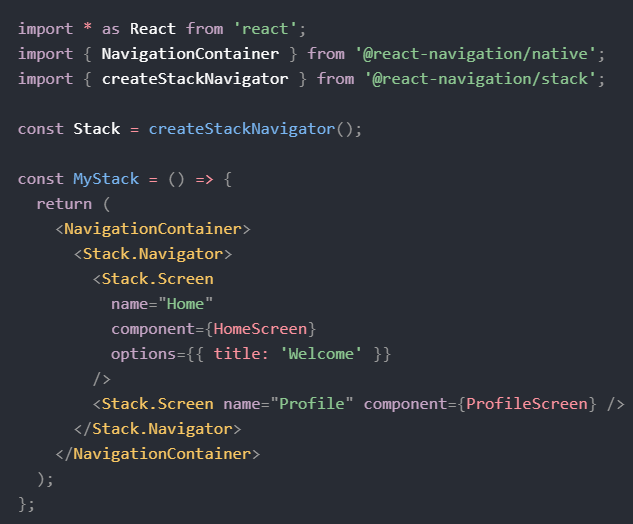
\includegraphics[width=\linewidth]{OpzettenNavigatieReactNative.png}
    \caption{Opzetten navigatie in een React Native applicatie. Bron: reactnative.dev/docs/navigation}
    \label{fig:opzettenNavigatieReactNative}
\end{figure}

Vervolgens moet er vastgelegd worden naar welke pagina er genavigeerd moet worden bij de uitvoering van een bepaald actie, zoals bv de klik op een bepaalde knop. Om dit mogelijk te maken krijgt elke component die een pagina voorstelt een attribuut navigation mee. In dit attribuut zitten methodes van de library die het navigeren tussen de verschillende pagina's mogelijk maakt. De opzet van een simpele navigatie is te zien in figuur \ref{fig:navigerenReactNative}. 

Zoals eerder vermeld heeft de library zeer veel mogelijkheden en levert het een navigatie af die native aanvoelt voor de gebruiker. Om dit te bereiken beschikt React Native Navigation ook over verschillende packages die o.a. tabs en drawer functionaliteit aanbieden. Dit zijn twee populaire manieren om te navigeren binnen een applicatie. Door dit aan te bieden in een package moet de ontwikkelaar niet helemaal zelf deze functionaliteit gaan uitwerken en wordt de standaard die de gebruiker gewoon is van native applicaties geëvenaard.

\begin{figure}
    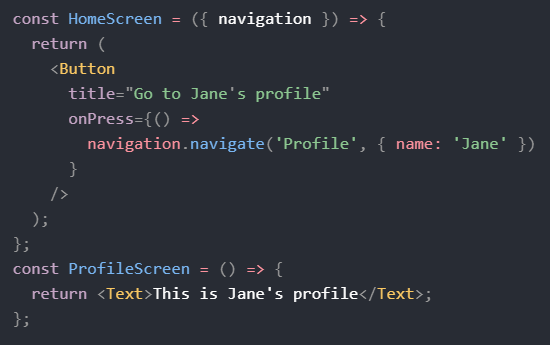
\includegraphics[width=\linewidth]{NavigerenPaginasReactNative.png}
    \caption{Navigeren naar een andere pagina in React Native. Bron: reactnative.dev/docs/navigation}
    \label{fig:navigerenReactNative}
\end{figure}

\subsubsection{Flutter}
\label{subsubsec:navigatieFlutter}

Flutter maakt voor de navigatie binnen een applicatie gebruik van de klasse Navigator. Deze klasse op zich is ook een widget, de bouwstenen van een applicatie in Flutter. De verschillende pagina's en schermen van een applicatie worden routes genoemd. Deze routes worden op een stack geplaatst, die de volgorde van de routes bijhoudt. Er zijn twee verschillende aanpakken van navigatie binnen Flutter: de ene is gebaseerd op een vaste volgorde waar alle schermen elkaar opvolgen en de andere laat de ontwikkelaar toe om op aangepaste wijze te navigeren tussen verschillende pagina's. Beide aanpakken worden in de volgende paragrafen verder besproken. 

De eerste aanpak laat de gebruiker toe om in een vaste volgorde door de applicatie te navigeren. Dit is voornamelijk belangrijk als de gebruiker terug wil gaan naar het vorige scherm. In dit geval is het alleen maar logisch om naar de vorige route in de stack te gaan. Het is ook meteen de meest eenvoudige vorm van navigatie. Als de gebruiker naar een andere pagina navigeert wordt deze bovenaan de stack geplaatst. Indien de gebruiker terug wenst te gaan wordt de bovenste route terug verwijderd van de stack en komt de gebruiker op de vorige pagina terecht.

De tweede aanpak is een iets gecompliceerdere aanpak. Deze volgt geen logische volgorde maar wel de volgorde die vastgelegd is door de ontwikkelaar. De aanpak berust op een Navigator.pages object. Hieraan kunnen de verschillende pagina's toegevoegd worden. Vervolgens zal de Navigator dit Navigator.pages object omzetten in een stack van routes. Indien een nieuwe pagina wordt toegevoegd aan Navigator.pages dan wordt de stack ook geüpdate. 

\begin{figure}
    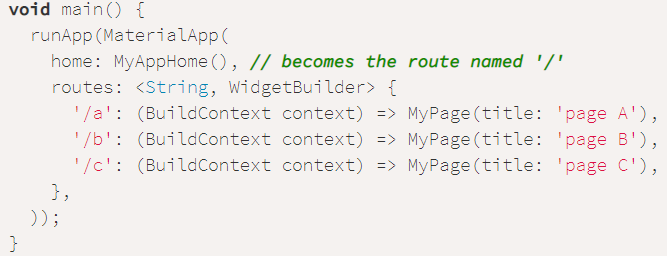
\includegraphics[width=\linewidth]{NamedRoutesFlutter.png}
    \caption{Opzetten navigatie met benoemde routes in Flutter. Bron: \textcite{Flutter.dev2020}}
    \label{fig:namedRoutesFlutter}
\end{figure}

\begin{figure}
    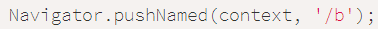
\includegraphics[width=0.5\linewidth]{UseNamedRouteFlutter.png}
    \caption{Benoemde route tonen in Flutter. Bron: \textcite{Flutter.dev2020}}
    \label{fig:useNamedRoutesFlutter}
\end{figure}

Een applicatie kan uit zeer veel verschillende schermen bestaan. Om de navigatie ertussen overzichtelijk te houden voor de ontwikkelaar beschikt Flutter over een functie om de routes een naam te geven. Vervolgens kan de pagina aan de hand van zijn naam getoond worden. In figuur \ref{fig:namedRoutesFlutter} is de definitie van een map te zien die de naam van een route bevat en de builder die de route effectief zal tonen op het scherm. In figuur \ref{fig:useNamedRoutesFlutter} is te zien hoe de route effectief getoond kan worden. Uit de naam van de methode wordt duidelijk dat ook deze methode gebruik maakt van een stack voor de navigatie. De nieuwe route wordt bovenop de stack geplaatst.

Beide methodes maken dus gebruik van dezelfde stack en kunnen dus ook door elkaar gebruikt worden. Dit is een logische aanpak, aangezien een logische volgorde in een applicatie absoluut noodzakelijk is. Indien een gebruiker terug wil gaan is het alleen logisch om naar de vorige stap te gaan, ongeacht welke methode gebruikt werd om naar de huidige pagina te navigeren. 

Verder is het in Flutter mogelijk om een route een waarde te laten terug geven. Dit is bijvoorbeeld handig indien de gebruiker op oké moet klikken alvorens er naar het volgende scherm gegaan kan worden. Indien de gebruiker uit dit scherm gaat door de terug knop van het systeem te gebruiken is de waarde die teruggegeven wordt null en zal het volgende scherm dus niet getoond worden.

Tot slot geeft de Navigator klasse de ontwikkelaar ook de mogelijkheid om popups te tonen op het scherm. Dit zijn schermen die niet de volledig oppervlakte van het scherm in nemen en dus nog een deel van het onderliggende scherm tonen. Het onderliggende scherm wordt echter geblokkeerd, de gebruiker kan dus enkel binnen de popup input geven. Deze popups gedragen zich verder als een normale route, de navigatie naar een popup en er weg van is dus exact hetzelfde.

\subsubsection{Vergelijking navigatie}
\label{subsubsec:vglNavigatie}

Beide frameworks hebben hun eigen techniek om de navigatie aan te pakken. Het grootste verschil tussen beiden is dat React Native gebruik maakt van een library, waar Flutter gebruik maakt van een widget. Dit verschil vloeit voort uit het fundamentele verschil in aanpak tussen beide frameworks. De oorzaak is dat React Native voor een heel groot deel door de community onderhouden wordt. Onder andere de library voor navigatie komt voort uit de community en zit dus niet standaard in React Native, waar dit bij Flutter wel standaard beschikbaar is.

Voor de volgorde van de navigatie bij te houden maken beide frameworks gebruik van een stack. Ze zijn dus beide in staat om terug te gaan naar de vorige pagina. Bij React Native moet elke pagina echter wel steeds benaamd worden om er naar toe te kunnen navigeren, waar het bij Flutter mogelijk is om op voorhand een vaste volgorde te definiëren.

In het gevoel voor de gebruiker is er echter geen verschil tussen beide frameworks. Beide frameworks leveren een navigatie af die overeen komt met de native navigatie. Verder kan de ontwikkelaar bij beide de overgang tussen de verschillende pagina's aanpassen om te voldoen aan de uitstraling die de app wilt geven. 

Er kan besloten worden dat er op het vlak van navigatie geen duidelijk beter framework is. Er is een verschil tussen de manier waarop de ontwikkelaar de navigatie implementeerd, maar voor de gebruiker heeft de navigatie met beide frameworks hetzelfde native gevoel.





% Voeg hier je eigen hoofdstukken toe die de ``corpus'' van je bachelorproef
% vormen. De structuur en titels hangen af van je eigen onderzoek. Je kan bv.
% elke fase in je onderzoek in een apart hoofdstuk bespreken.

%\input{...}
%\input{...}
%...

%%=============================================================================
%% Conclusie
%%=============================================================================

\chapter{Conclusie}
\label{ch:conclusie}

% TODO: Trek een duidelijke conclusie, in de vorm van een antwoord op de
% onderzoeksvra(a)g(en). Wat was jouw bijdrage aan het onderzoeksdomein en
% hoe biedt dit meerwaarde aan het vakgebied/doelgroep? 
% Reflecteer kritisch over het resultaat. In Engelse teksten wordt deze sectie
% ``Discussion'' genoemd. Had je deze uitkomst verwacht? Zijn er zaken die nog
% niet duidelijk zijn?
% Heeft het onderzoek geleid tot nieuwe vragen die uitnodigen tot verder 
%onderzoek?


In het vorige hoofstuk werd vertrokken van een grote lijst (sectie \ref{subsec:lijstPopulairsteFrameworks} met cross-platform frameworks die in 2019 en 2020 gebruikt werden door ontwikkelaars van overal ter wereld. Al de frameworks (op 2 na die duidelijk niet voldoen aan de eis om in de toekomst een goede keuze te zijn) die voorkwamen in de lijst werden kort besproken (sectie \ref{subsec:achtergrondFrameworks}. Vervolgens werden deze frameworks afgetoetst tegen de eisen die gesteld werden aan het framework in sectie \ref{sec:aftoetsenEisen}. Na het aftoetsen van de frameworks tegenover de eisen waren er slechts twee frameworks die op dit moment voldeden aan alle eisen: React Native en Flutter.

\section{Conclusies vergelijkingen React Native en Flutter}
\label{sec:conclusieVgl}

Tijdens het vergelijken van React Native en Flutter werd het duidelijk dat beide frameworks enkele verschillen vertonen maar dat de concepten waarop het famework gebaseerd is grotendeels gelijk zijn. Zo beschikken beide frameworks over een manier om aan hot reloading te doen, hebben ze beiden de mogelijkheid om toegang te verkrijgen tot de native API's en is er zelfs geen noemenswaardig verschil te merken in de prestaties van een app die geschreven is met React Native of één met Flutter. In de volgende paragrafen worden de conclusies van de verschillende onderzoekspunten gegeven.

\subsubsection{Taal framework}

Een eerste punt van vergelijking was de taal van het framework. Uit deze vergelijking kan besloten worden dat beide frameworks gebaseerd zijn op een taal die veel mogelijkheden bezit. React Native is gebaseerd op JavaScript, dat al een pak langer bestaat dan Dart(de taal van Flutter). Hierdoor is er veel meer documentatie beschikbaar, zijn er meer externe libraries van de community om vaste taken over te nemen en zijn er meer oplossingen beschikbaar voor veel voorkomende problemen. Op dit moment is React Native dus een betere optie voor de meeste ontwikkelaars, zeker indien er reeds een basiskennis React aanwezig is. Dart heeft echter als voordeel dat de bron code gecompiled kan worden naar native machine code, wat een groot voordeel kan opleveren in sommige gevallen. Indien de taal dus aan maturiteit en populariteit wint in de komende jaren zou de conclusie van het onderzoek op dit punt dus wel in het voordeel van Dart en dus Flutter kunnen overslaan.

\subsubsection{Navigatie binnen de applicatie}

Op het vlak van navigatie waren er enkele verschillen in de technologie voor de ontwikkelaar. Zo wordt er bij React Native een beroep gedaan op een library van de community, waar dit bij Flutter standaard in het framework aanwezig is. Voor de gebruiker is er echter geen enkel verschil waarneembaar en werkt de navigatie van de applicatie net zoals deze van een native applicatie. Op dit gebied is er dus geen onderscheid te maken tussen beide frameworks.

\subsubsection{Toegang native API's}

Een belangrijk punt voor een framework is dat het de ontwikkelaar toegang geeft tot de native API's indien dit nodig is. Zowel React Native als Flutter zijn hiertoe in staat. Kennis van native code is hier wel van essentieel belang om gebruik te kunnen maken van deze eigenschap. Ook hier is echter geen onderscheid merkbaar tussen beide frameworks.

\subsubsection{Opbouw UI}

Als er naar de opbouw van de UI gekeken wordt is er wel een groot verschil tussen beide frameworks. Hoewel de opbouw van de UI met Flutter gebaseerd is op bepaalde concepten van React is het uiteindelijke resultaat een groot verschil met React Native.

De twee frameworks maken allebei gebruik van bouwstenen, die door ze te combineren de UI voorstellen. Bij React Native zijn dit React componenten, bij Flutter zijn het widgets. Beiden kunnen volledig gestijld worden naar de smaak van de ontwikkelaar. 

De data flow van de ene component naar de andere bij React Native is exact dezelde als deze tussen twee widgets. Data vloeit van de ouder naar het kind, in de omgekeerde richting worden callback functies gebruikt.

Het verschil in de opbouw van de UI tussen beide frameworks zit niet in wat de ontwikkelaar ziet of moet doen, maar gebeurd op de achtergrond. React Native componenten worden met behulp van JavaScript bruggen gemapt naar hun overeenkomstige native componenten 'at runtime'. De bron code van een Flutter applicatie wordt echter omgezet naar native machine code, waardoor de gedefinieerde widgets blijven bestaan. De widgets die de ontwikkelaar maakt krijgt de gebruiker dus ook effectief te zien. 

De aanpak van React Native om de componenten te mappen naar echte native componenten heeft één groot voordeel ten opzichte van de aanpak van Flutter: doordeze mapping naar native componenten wordt de weergave van deze componenten automatisch mee aangepast indien er een update van de stijl van de UI van een platform uitgebracht wordt. Bij Flutter moet er gewacht worden totdat deze nieuwe stijl is overgenomen in de widgets. 

Ook op dit punt is er geen duidelijk verschil tussen welk van de twee frameworks de betere keuze is. Dat er verschillen zijn in aanpak is duidelijk, maar geen van beide aanpakken heeft een duidelijk voordeel ten opzichte van de andere. 

\subsubsection{Ondersteuning andere platformen}

Op het moment van schrijven van deze studie heeft Flutter nog geen ondersteuning voor andere platformen dan Android en iOS. React Native heeft deze wel reeds en heeft dus op dit vlak een streepje voor.

\subsubsection{Prestaties}

Als laatste punt van de vergelijking werden de prestaties van beide frameworks vergeleken. Voor deze vergelijking werd een beroep gedaan op de studie van \textcite{Fentaw2020}. Er werd geen eigen prestatiestudie gedaan omdat dit buiten de opzet van deze studie lag. Uit deze studie kon geconcludeerd worden dat er op bepaalde taken door het eerste framework beter gepresteerd wordt, op andere taken scoort het tweede framework beter en op andere taken scoren ze gelijkaardig. Over de algemene lijn gezien is er dus geen noemenswaardig verschil tussen beide frameworks op het vlak van prestaties.

\section{Algemene conclusie}
\label{sec:AlgemeneConclusie}

In de vorige sectie werd de conclusie per onderzoeksdeel gegeven. In deze sectie worden deze afzonderlijke conclusies gecombineerd tot een algemene conclusie en een antwoord op de onderzoeksvraag.

Uit de conclusies in de vorige sectie blijkt duidelijk dat er geen afgetekend verschil is tussen welk framework de beste keuze is. Beide frameworks zijn ongeveer even populair (zie figuur \ref{fig:frameworkPopularity}), beschikken over dezelfde functionaliteiten en er is geen noemenswaardig verschil in prestaties tussen beide frameworks. Er kan dus besloten worden dat er op dit moment puur technologisch gezien geen beste keuze is tussen beide frameworks.

Indien er echter verder gekeken wordt dan het puur technologische en ook de ondersteuning, documentatie en de volwassenheid van het framework en de taal waarop het framework gebaseerd is dan moet er geconcludeerd worden dat op dit moment React Native de betere keuze is. 

Als er specifiek gekeken wordt welk framework de beste keuze is voor het Mobile, Web en IoT-team van delaware (waarvoor deze studie in de eerste plaats geschreven werd) dan kan er ook verder gekeken worden dan enkel de vergelijkingspunten die reeds in deze studie aan bod kwamen. Onder meer de ervaring van het team speelt dan een grote rol. Aangezien het team voor de ontwikkeling van webapplicaties reeds gebruik maakt van React is de stap naar React Native een keuze die natuurlijker zal aanvoelen dan de overgang naar Flutter (en dus Dart). 

Verder is het de bedoeling om mobiele applicaties te gaan schrijven voor de B2B-markt. Waar Windows het in de gewone markt heeft moeten afleggen tegenover Android en iOS is dit op de B2B-markt wel nog aanwezig. Aangezien Flutter hier op het moment van schrijven nog geen ondersteuning voor aanbiedt is React Native de beste optie om de komende jaren mee aan de slag te gaan voor het schrijven van mobiele applicaties voor de B2B-markt.

\section{Verder onderzoek}
\label{sec:verderOnderzoek}

Tijdens het opstellen van de lijst van frameworks kwamen enkele frameworks aan bod die nog maar zeer recent ontstaan zijn. Zo is er bijvoorbeeld de ondersteuning voor cross-platform applicatieontwikkeling van Kotlin en de opvolger van Xamarin, .NET MAUI. Beide frameworks hebben heel veel potentieel en indien deze studie op een later tijdsstip opnieuw uitgevoerd zou worden kan het zijn dat deze wel zouden voldoen aan de eisen en eventueel zelfs een betere keuze zouden zijn dan React Native of Flutter. Op het moment van schrijven is de ondersteuning van cross-platform in Kotlin echter nog experimenteel en zit .NET MAUI nog in de beta fase waardoor ze het beiden moeten afleggen tegen React Native en Flutter.

Indien dit onderzoek op een later moment nog eens opnieuw gevoerd wordt kan het ook heel goed zijn dat er nog andere frameworks zijn bijgekomen die eventueel beter zijn dan de frameworks die hier besproken werden. Het is dus belangrijk om als team zich niet vast te pinnen op deze studie, maar zelf een gelijkaardige studie uit te voeren op het moment dat er een beslissing gemaakt moet worden.

Tot slot is er nog een grote mogelijkheid om de prestaties van Kotlin Multiplatform en .NET MAUI te vergelijken met deze van React Native en Flutter eens beide frameworks beschibaar zijn. 

Studies zoals deze zullen echter steeds maar een bepaalde tijd relevant zijn door het snel veranderende landschap in de wereld van cross-platform applicatie ontwikkeling. Ze zijn dus alleen maar relevant indien het, zoals bij deze studie het geval was, een specifiek doel dient voor een bepaalde doelgroep.








%%=============================================================================
%% Bijlagen
%%=============================================================================

\appendix
\renewcommand{\chaptername}{Appendix}

%%---------- Onderzoeksvoorstel -----------------------------------------------

\chapter{Onderzoeksvoorstel}

Het onderwerp van deze bachelorproef is gebaseerd op een onderzoeksvoorstel dat vooraf werd beoordeeld door de promotor. Dat voorstel is opgenomen in deze bijlage.

% Verwijzing naar het bestand met de inhoud van het onderzoeksvoorstel
%---------- Inleiding ---------------------------------------------------------

\section{Introductie} % The \section*{} command stops section numbering
\label{sec:introductie}

Bij het ontwikkelen van een chatbot komen zeer veel moeilijkheden kijken. Eén van deze moeilijkheden is dat een chatbot afhankelijk is van wat een gebruiker ingeeft. Door het feit dat er oneindig veel mogelijke waarden zijn waar de chatbot mee aan de slag moet gaan is het een grote uitdaging om de input van de gebruiker correct te gaan interpreteren en correct te gaan reageren op deze input. Het is dus snel duidelijk dat er zich op beide vlakken vele fouten kunnen voordoen. Om een chatbot te testen moet op dit moment een persoon effectief deze waarden gaan ingeven en gaan kijken wat de reactie van de chatbot is. Deze studie zal zich richten op een onderzoek naar reeds bestaande manieren om regressietesten te gaan schrijven en de ontwikkeling van een test die een goede basis zal vormen waar Clever mee aan de slag kan om hun chatbots verder te gaan testen. Het doel van deze studie is dus duidelijk: een concrete aanbeveling doen van een framework dat in staat is om op een gebruiksvriendelijke manier onderhoudbare regressietesten te gaan schrijven. De onderzoeksvraag voor deze studie luidt als volgt: welk reeds bestaand framework levert de meest onderhoudbare oplossing om op een gebruiksvriendelijke manier regressietesten te schrijven voor een chatbot? Er zijn echter ook nog enkele deelonderzoeksvragen, die ook zeker niet vergeten mogen worden. Een eerste deelvraag is wat de beste methode is om regressietesten op een zo goedkoop mogelijke en zo min mogelijk resource-intensieve manier te gaan uitvoeren. Een volgende vraag is welke van deze methodes bruikbaar zijn om te gaan gebruiken voor het schrijven van regressietesten voor chatbots. 

%---------- Stand van zaken ---------------------------------------------------

\section{Literatuurstudie}
\label{sec:literatuurstudie}

\subsection{Definitie van regressietesten}

Volgens \textcite{EngstroemRuneson2010} is regressietesten het hertesten van voordien werkende software nadat er wijziging zijn doorgevoerd om te verzekeren dat niet aangepaste software nog steeds werkt als voordien. In een onderzoek naar de definitie van regressietesten in de opinie van experts uit de industrie, kwamen \cite{Minhas2017} tot de conclusie dat de industrie regressietesten op 2 manieren zou beschrijven. Enerzijds is regressietesten een activiteit die vertrouwen geeft over wat er is uitgevoerd en die zekerheid geeft dat er niks is kapot gemaakt. Anderzijds is regressietesten een activiteit die er voor zorgt dat alles correct blijft werken na een wijziging in het systeem en het is een garantie dat het systeem ook in de toekomst zal blijven werken.

\subsection{Activiteiten bij regressietesten}

Volgens  \textcite{AhlamAnsari2016} worden er steeds 3 activiteiten uitgevoerd alvorens de regressietesten effectief te laten runnen:

\begin{itemize}
    \item Selectie van de test case: de relevante test cases voor een specifiek deel van de applicatie of de uitgevoerde aanpassingen.
    \item Minimaliseren van de test case: het aantal test cases wordt beperkt door test cases die hetzelfde testen te verwijderen. 
    \item Prioriteit stellen van bepaalde test cases: de volgorde bepalen waarin de test cases zullen uitgevoerd worden zodat de kans om fouten op te sporen gemaximaliseerd wordt.
\end{itemize}

Deze 3 stappen zijn zeer belangrijk: naarmate een applicatie groter wordt zal ook de test suite (de verzamelig van alle testen) zeer groot worden. Deze kunnen niet allemaal steeds opnieuw uitgevoerd worden (dit zou veel te lang duren en dus ook te veel geld kosten). Er wordt dus telkens slechts een deel van de beschikbare test cases uitgevoerd. De testen moeten echter wel nog steeds zekerheid geven dat de code geen fouten bevat. Het is dus essentieel om een goede selectie van test cases te maken. 

Volgens \textcite{PrashantMalangave2015} is de beste manier om aan 'Test prioritization' te doen kijken naar de code coverage (hoeveel procent van de code effectief getest wordt door deze test). Uit de geselecteerde test cases is de beste strategie om eerst deze met de grootste code coverage te gaan kiezen doordat er meer fouten gevonden kunnen worden als er meer code getest wordt.

\subsection{Combinatorial interaction regression test (CIT)}

Een mogelijke oplossing voor het verkleinen van het aantal test cases dat gebruikt moet worden is volgens \textcite{Qu2014} Combinatorial interaction testing (CIT). Dit is een techniek die gebruik maakt van parameter interacties om fouten te ontdekken, waardoor ook de interactie tussen verschillende compononenten van het systeem behandeld wordt \autocite{Brcic2013}.

% Voor literatuurverwijzingen zijn er twee belangrijke commando's:
% \autocite{KEY} => (Auteur, jBij het aartal) Gebruik dit als de naam van de auteur
%   geen onderdeel is van de zin.
% \textcite{KEY} => Auteur (jaartal)  Gebruik dit als de auteursnaam wel een
%   functie heeft in de zin (bv. ``Uit onderzoek door Doll & Hill (1954) bleek
%   ...'')

%---------- Methodologie ------------------------------------------------------
\section{Methodologie}
\label{sec:methodologie}

Om een goed beeld te krijgen van de reeds bestaande oplossingen voor regressietesten zal er eerst hierover een grondige tudie gevoerd worden. Vervolgens zal er een grondige studie gedaan worden naar de werking van chatbots. Na afloop van beide studies zal er bekeken worden hoe de bestaande oplossingen voor regressietesten geïmplementeerd kunnen worden om regressietesten voor chatbots te gaan ontwikkelen. Om te testen of de aangewezen methodes voor het schrijven van regressietesten effectief bruikbaar zijn bij het testen van chatbots zal er een test case uitgewerkt worden. Aan de hand van de resultaten van deze test case kan er vervolgens bepaald worden of deze methodes effectief een meerwaarde bieden. Voor de gebruiksvriendelijkheid van de methode te testen zal er een klein experiment uitgevoerd worden bij Clever en achteraf een vragenlijst. Op deze manier kan bepaald worden of de voorgestelde methode effectief bruikbaar is en een meerwaarde zal kunnen bieden in de toekomst. 


%---------- Verwachte resultaten ----------------------------------------------
\section{Verwachte resultaten}
\label{sec:verwachte_resultaten}

De lijn van verwachting voor dit onderzoek is dat er een concreet voorstel zal uit voortvloeien om met een bepaalde methode aan de slag te gaan. De kans is echter groot dat er op dit moment nog geen framework beschikbaar is dat helemaal zal voldoen aan de noden van Clever. Gezien het feit dat het ontwikkelen van een test framework niet hoort tot de scope van dit onderzoek zal er in dit geval geen kant en klare oplossing zijn. Wel kan het resultaat van dit onderzoek leiden tot een beter inzicht van hoe er aan de slag kan gegaan worden met de reeds bestaande frameworks.

%---------- Verwachte conclusies ----------------------------------------------
\section{Verwachte conclusies}
\label{sec:verwachte_conclusies}

De verwachte conclusie is dat het schrijven van regressietesten voor chatbots geen sinecure is. Door de enorme hoeveelheid mogelijke input zal nooit de volledige chatbot telkens opnieuw getest kunnen worden. Wat wel mogelijk zal blijken is dat de taalherkenning en de meest voorkomende vragen die de chatbot zal moeten beantwoorden getest zullen kunnen worden. Een aanrading van een framework zal er waarschijnlijk wel inzitten, maar een proof of concept opleveren zal alleen lukken indien er een gratis framework beschikbaar is. Een laatste conclusie zal echter zijn dat het testen van chatbots een tijdsintensieve gebeurtenis zal blijven en dat er nog zeer veel ruimte zal zijn voor verbetering op het vlak van gebruiksvriendelijkheid.



%%---------- Andere bijlagen --------------------------------------------------
% TODO: Voeg hier eventuele andere bijlagen toe
%\input{...}

%%---------- Referentielijst --------------------------------------------------

\printbibliography[heading=bibintoc]

\end{document}
